% Resultat 1/5 
%Å analysere gjør du ved å redegjøre, forklare og vurdere funnene dine. Analysedelen av oppgaven blir ofte kalt resultater, slik som i IMRoD-modellen.

%I kvantitative studier vil du kanskje i tillegg til å presentere funnene skriflig, bruke figurer og tabeller for å gi leseren en oversikt og innsikt i hva du har gjort.
%I empirisk baserte studier vil analysene handle om å beskrive og tolke. Mange vil ofte drøfte enkeltfunnene i dette kapitlet og ta for seg mer overordnede funn i drøftingskapitlet.
%Et lurt tips for å finne ut hvordan du kan skrive ditt analysekapittel, er å se hvordan det er gjort i andre oppgaver på tilsvarende nivå fra samme felt.

\section{Resultater}
\label{part:results}

Det ble trent opp to modeller, en RetinaNet-modell og en YOLOv4-modell. Se figur \ref{fig:inference} og \ref{fig:yolo_inference}. Dataen av torsk bestod av tre kanaler, og hadde størrelsen 1920 $\times$ 1080. Bildene av sei bestod av kun en kanal, og hadde størrelsen 640 $\times$ 480. Se figur \ref{fig:data}.

%A classification accuracy of 94.3 \% was achieved when classifying only the 16 fish species which we focussed on for this trial. All other evaluations include the other species class which contains a number of fish species which are non-relevant to the research goals, but can be encountered while underwater sampling. The re- sults obtained by the different model configurations are summa- rized in Table 2. The model based on ResNet (He et al., 2016) by cross-pooling activations from layer 4b15 and 4b20, with local region size of 3 and training of a linear SVM on top of the cross-pooled features, was able to achieve the highest classifica- tion accuracy of 89.0 \% if the other species class is included. A change to a local region size of 1 produces a slightly inferior result of 86.9 \% classification accuracy for all classes. In compari- son, the AlexNet and VGGNet model configurations produced significantly degraded results.

%Application of the linear SVM di- rectly to features from the Pool5 layer of the ResNet-152 model resulted in a classification accuracy of 71.49 \%, highlighting the improved performance produced by cross-layer pooling. We re- duced the dimensionality of the 3 local features in ResNet- 152b model from 9216 (3 3 1024) to 512 before cross-layer pooling using PCA. Dimensionality reduction can be useful in or- der to reduce the size of features from cross-layer pooling, allow- ing use of larger region sizes as well as more feature maps. Adapting a larger region size even with the use of PCA improved accuracy of the system due to availability of local context. 

%Further analysis of the accuracy of the four CNN models can be con- ducted using the precision and recall of the classifier. Recall and precision are a more informative way to judge the performance of a classifier, especially if the classes are skewed.


%The precision of a classifier is a measure of correctly classified images out of all the images predicted to belong to a specific class. Mathematically,

%In general, the precision and recall graphs confirm the classifi- cation accuracy levels shown in Table 2, with very few exceptions. In some cases, the ResNet-152 model with a 1 1 local region produces the best result, but these exceptions reflect the small dif- ference in the classification accuracy between the two sizes of lo- cal region. Precision is generally higher than recall, indicating that false negatives are more common than false positives. The precision graph shows high values for a number of individual species, indicating that the number of false positives is very low. The lesser precision in ...

\subsection{RetinaNet}

\begin{figure}[h!]
\begin{center} 
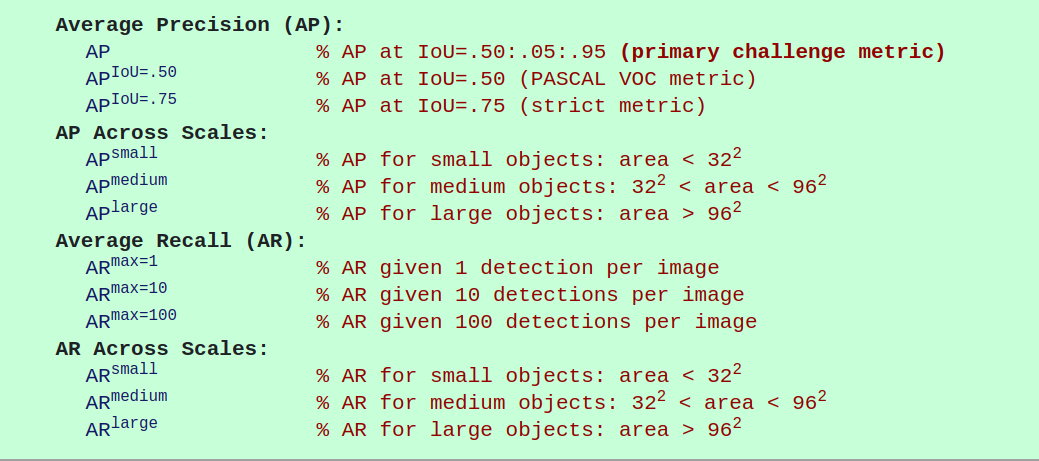
\includegraphics[scale=0.35]{figures/coco}
\caption{\small \sl Evalueringskortet til COCO. En modell som har blitt trent med vekter fra COCO kan evalueres etter dette kortet. \label{fig:coco}}
\end{center}
\end{figure}

AP står for «Average Precision», og AR står for «Average Recall». De er mål på hvor nøyaktig en deep learning-modell er. Se tabellene på side \pageref{tab:ap_retinanet}.

\begin{table}[]
\bigskip
\centering
\label{tab:ap_retinanet} 
\caption{AP (primary challenge metric) og Average Recall}
\begin{tabular}[t]{lccc}
\toprule
 Average Precision  (AP) @ [ IoU=0.50:0.95 & area=   all & maxDets=100 ] &= 0.285 \\
 Average Precision  (AP) @ [ IoU=0.50      & area=   all & maxDets=100 ] &= 0.663 \\
 Average Precision  (AP) @ [ IoU=0.75      & area=   all & maxDets=100 ] &= 0.200 \\
 Average Precision  (AP) @ [ IoU=0.50:0.95 & area= small & maxDets=100 ] &= 0.067 \\
 Average Precision  (AP) @ [ IoU=0.50:0.95 & area=medium & maxDets=100 ] &= 0.217 \\
 Average Precision  (AP) @ [ IoU=0.50:0.95 & area= large & maxDets=100 ] &= 0.402 \\
\midrule
 Average Recall     (AR) @ [ IoU=0.50:0.95 & area=   all & maxDets=  1 ] &= 0.038 \\
 Average Recall     (AR) @ [ IoU=0.50:0.95 & area=   all & maxDets= 10 ] &= 0.248 \\
 Average Recall     (AR) @ [ IoU=0.50:0.95 & area=   all & maxDets=100 ] &= 0.433 \\
 Average Recall     (AR) @ [ IoU=0.50:0.95 & area= small & maxDets=100 ] &= 0.139 \\
 Average Recall     (AR) @ [ IoU=0.50:0.95 & area=medium & maxDets=100 ] &= 0.352 \\
 Average Recall     (AR) @ [ IoU=0.50:0.95 & area= large & maxDets=100 ] &= 0.556 \\
 \bottomrule	
 \end{tabular}
\end{table}

\begin{table}[]
\bigskip
\centering
\caption{Evaluation results for bbox} 
\label{tab:bbox_retinanet} 
\begin{tabular}[t]{lccccc}
\toprule
   AP   &  AP50  &  AP75  &  APs  &  APm   &  APl    \\
 \midrule
 28.494 & 66.262 & 20.016 & 6.654 & 21.663 & 40.239 \\
 \bottomrule	
 \end{tabular}
\end{table}

\begin{table}[]
\bigskip
\centering
\label{tab:per-category_bbox_retinanet} 
\caption{Per-category bbox AP} 
\begin{tabular}[t]{lccc}
\toprule
 category     & AP     & category   & AP      \\
 \midrule
 atlantic\_cod & 23.077 & saithe     & 33.910 \\
 \bottomrule	
\end{tabular}
\end{table}

\subsubsection{COCO deteksjonsevaluering} 

Resultatene i tabell \ref{tab:ap_retinanet} kan sammenlignes med evalueringskortet i figur \ref{fig:coco}. Resultatene bør være bedre enn COCO-evalueringskortet. AP (primary challenge metric) bør være mer enn 0,5. RetinaNet-modellen har en AP lik 0,285. Se tabell \ref{tab:ap_retinanet}. AP for torsk var 23,1 \%, og 33,9 \% for sei. Se tabell \ref{tab:per-category_bbox_retinanet}.

%\begin{figure}[h!]
%\begin{center} 
%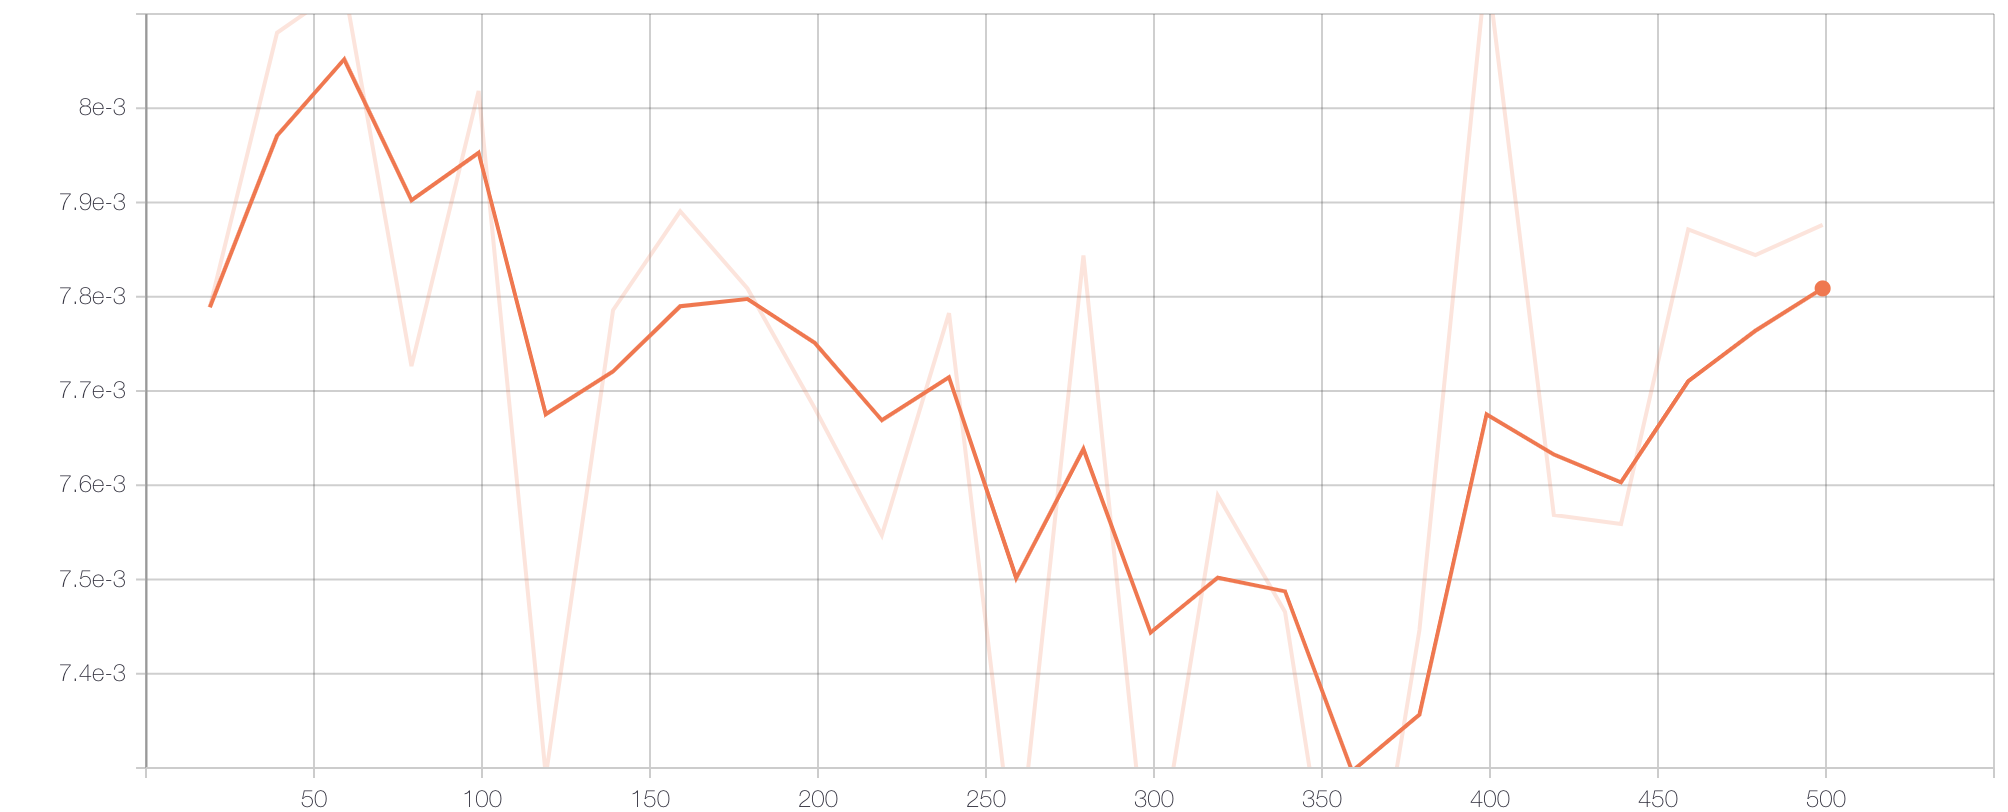
\includegraphics[scale=0.35]{figures/data_time_retinanet_1}
%\caption{\small \sl data time RetinaNet. \label{fig:data_time_retinanet}}
%\end{center}
%\end{figure}

%\begin{figure}[h!]
%\begin{center} 
%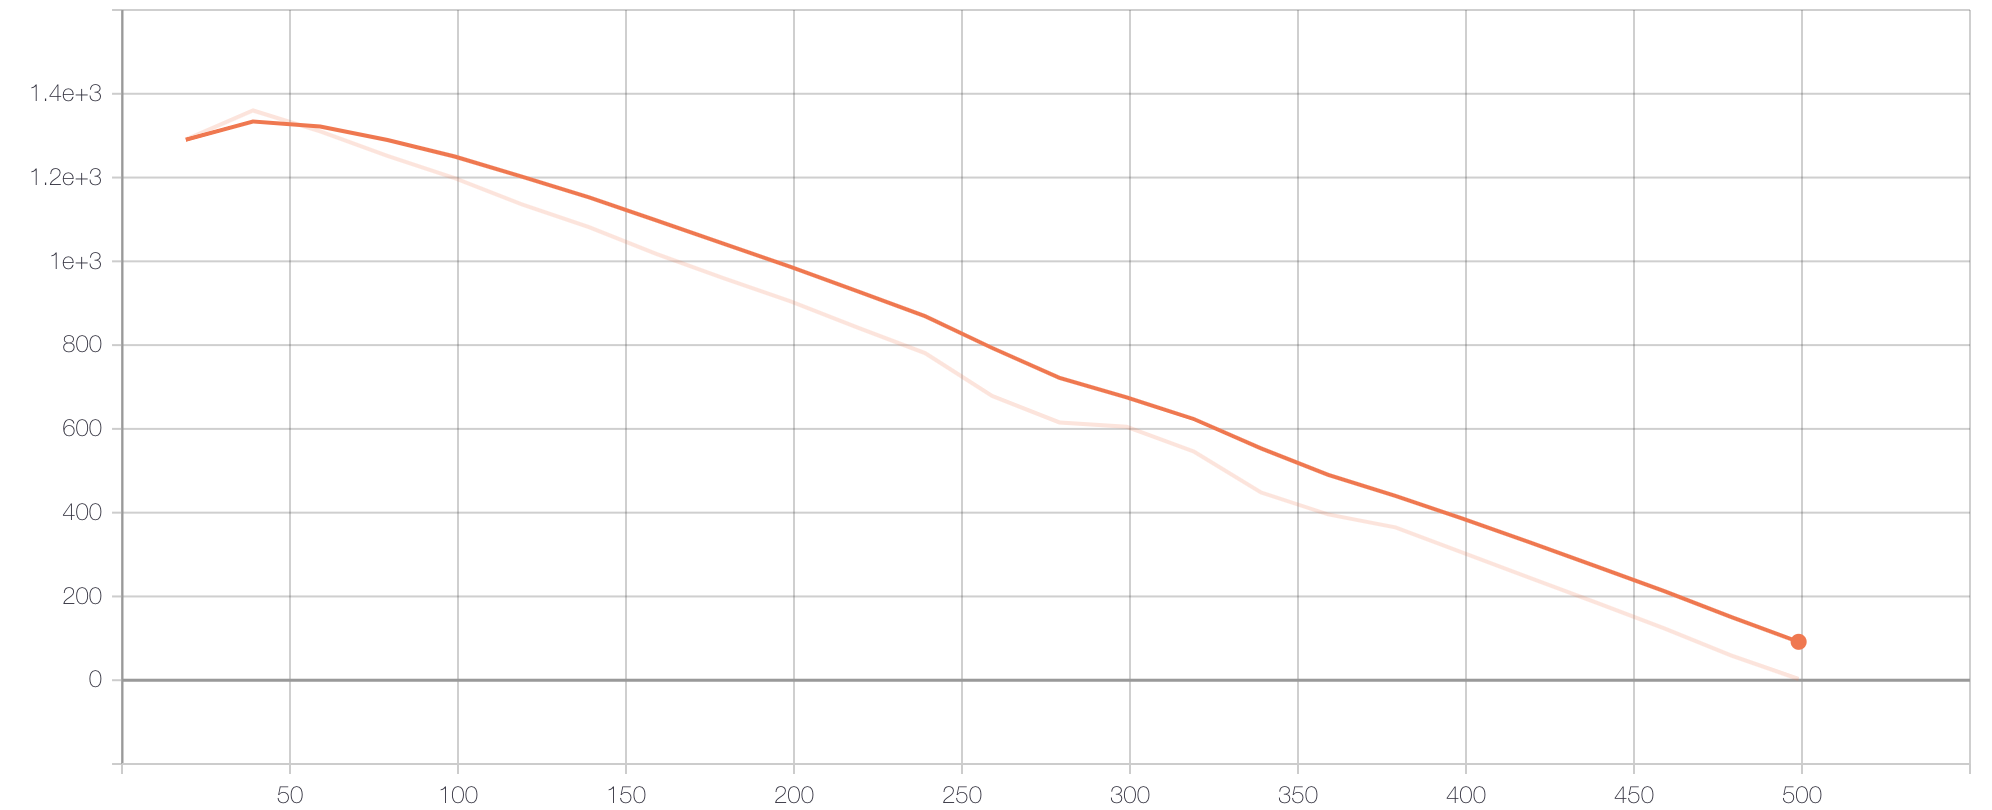
\includegraphics[scale=0.35]{figures/eta_seconds_retinanet_2}
%\caption{\small \sl eta seconds RetinaNet. \label{fig:eta_seconds_retinanet}}
%\end{center}
%\end{figure}

\subsubsection{TensorBoard resultater}

Alle grafene under er fra TensorBoard, et verktøy fra Google som er utviklet til å hjelpe dataforskere med å trene opp deep learning-modeller og dele resultatene til forsøkene deres. TensorBoard visualiserer maskinlæringseksperimenter og er egentlig laget for Google sin deep learning-rammeverk som heter Tensorflow, men PyTorch støtter også TensorBoard \cite{Oshri 2019}. Resultatene lastes opp med kommandoen \texttt{tensorboard dev upload --logdir logs --name 'TMAT3004' --description 'Bachelorprosjekt NTNU 2020'}.

I alle grafene fra TensorBoard, figur \ref{fig:loss_box_reg_retinanet}, \ref{fig:loss_cls_retinanet}, \ref{fig:lr_retinanet} og \ref{fig:total_loss_retinanet}, så er x-aksen tid i sekunder fra begynnelsen av forsøket, og y-aksen verdien til den spesifikke målingen. 

Den første grafen nedenfor er «loss bounding box». Dette er et mål på hvor tett modellen satt bounding box-ene rundt objektene som fantes i bildene den gjorde inferens på.

\begin{figure}[H]
\begin{center} 
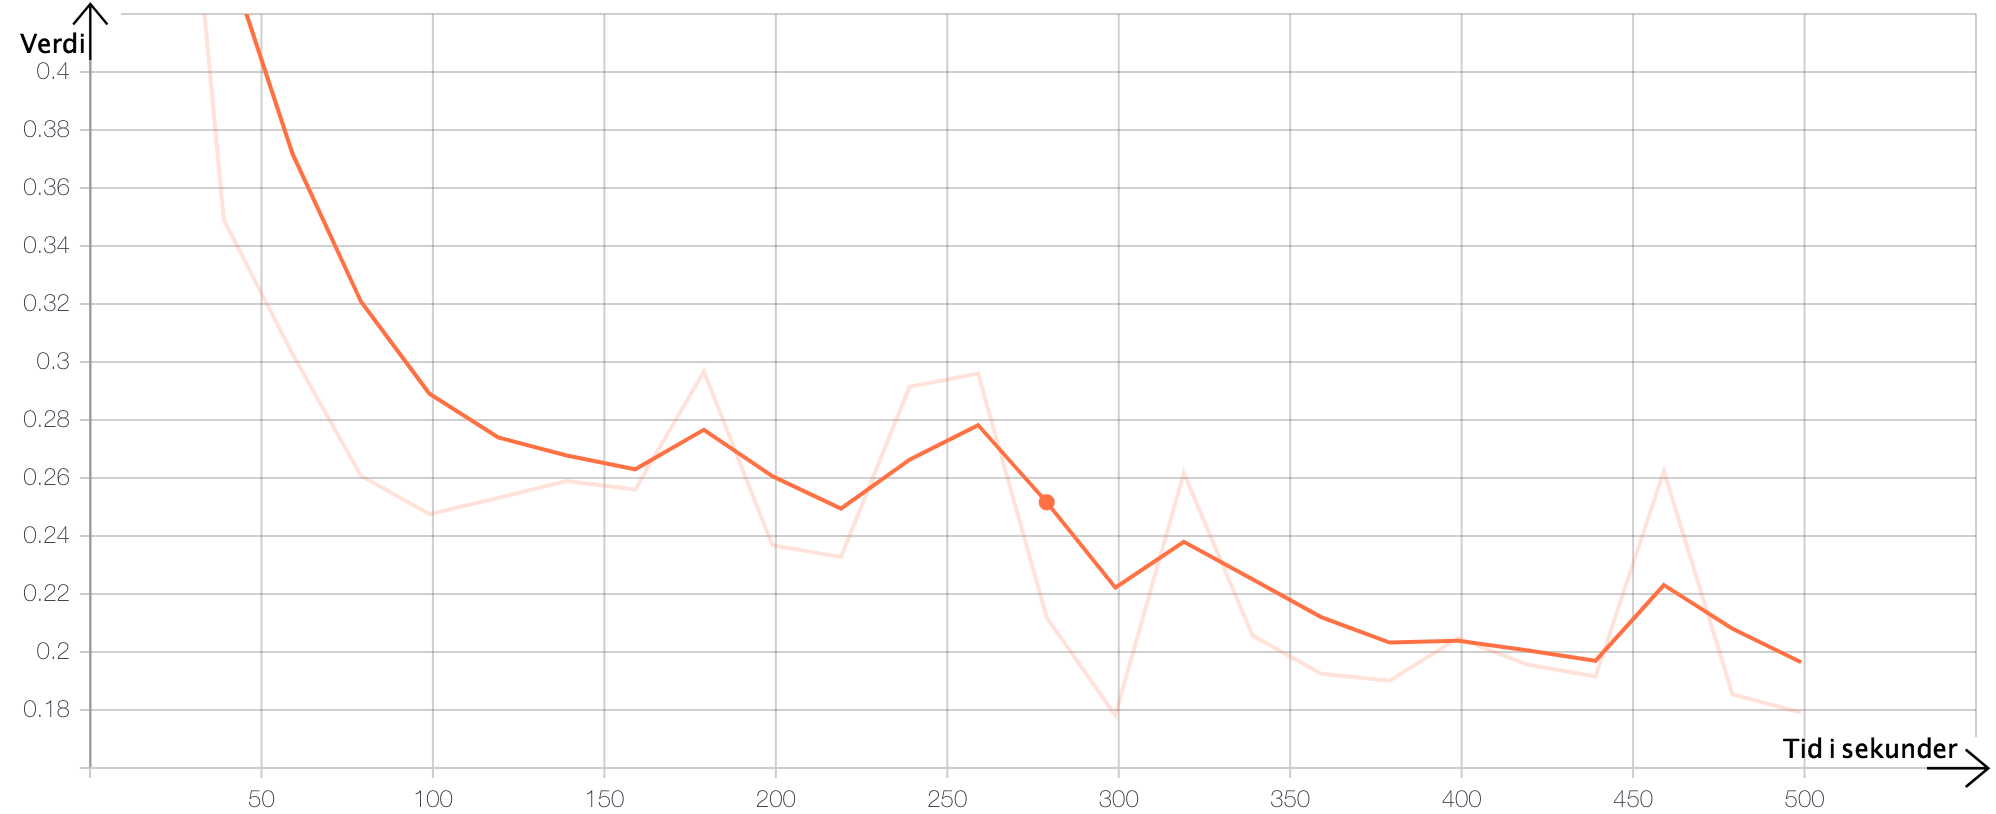
\includegraphics[scale=0.35]{figures/loss_box_reg_retinanet_3}
\caption{\small \sl «Loss bounding box» for RetinaNet. \label{fig:loss_box_reg_retinanet}}
\end{center}
\end{figure}

Neste graf viser «loss cls», eller «entropy loss». Entropy loss er et mål på hvor korrekt klassifiseringen av hver «bounding box» var. Hver «bounding box» kan inneholde en klasse, altså et objekt, eller være bakgrunn, og dermed være en boks som ikke inneholder en klasse.

\begin{figure}[H]
\begin{center} 
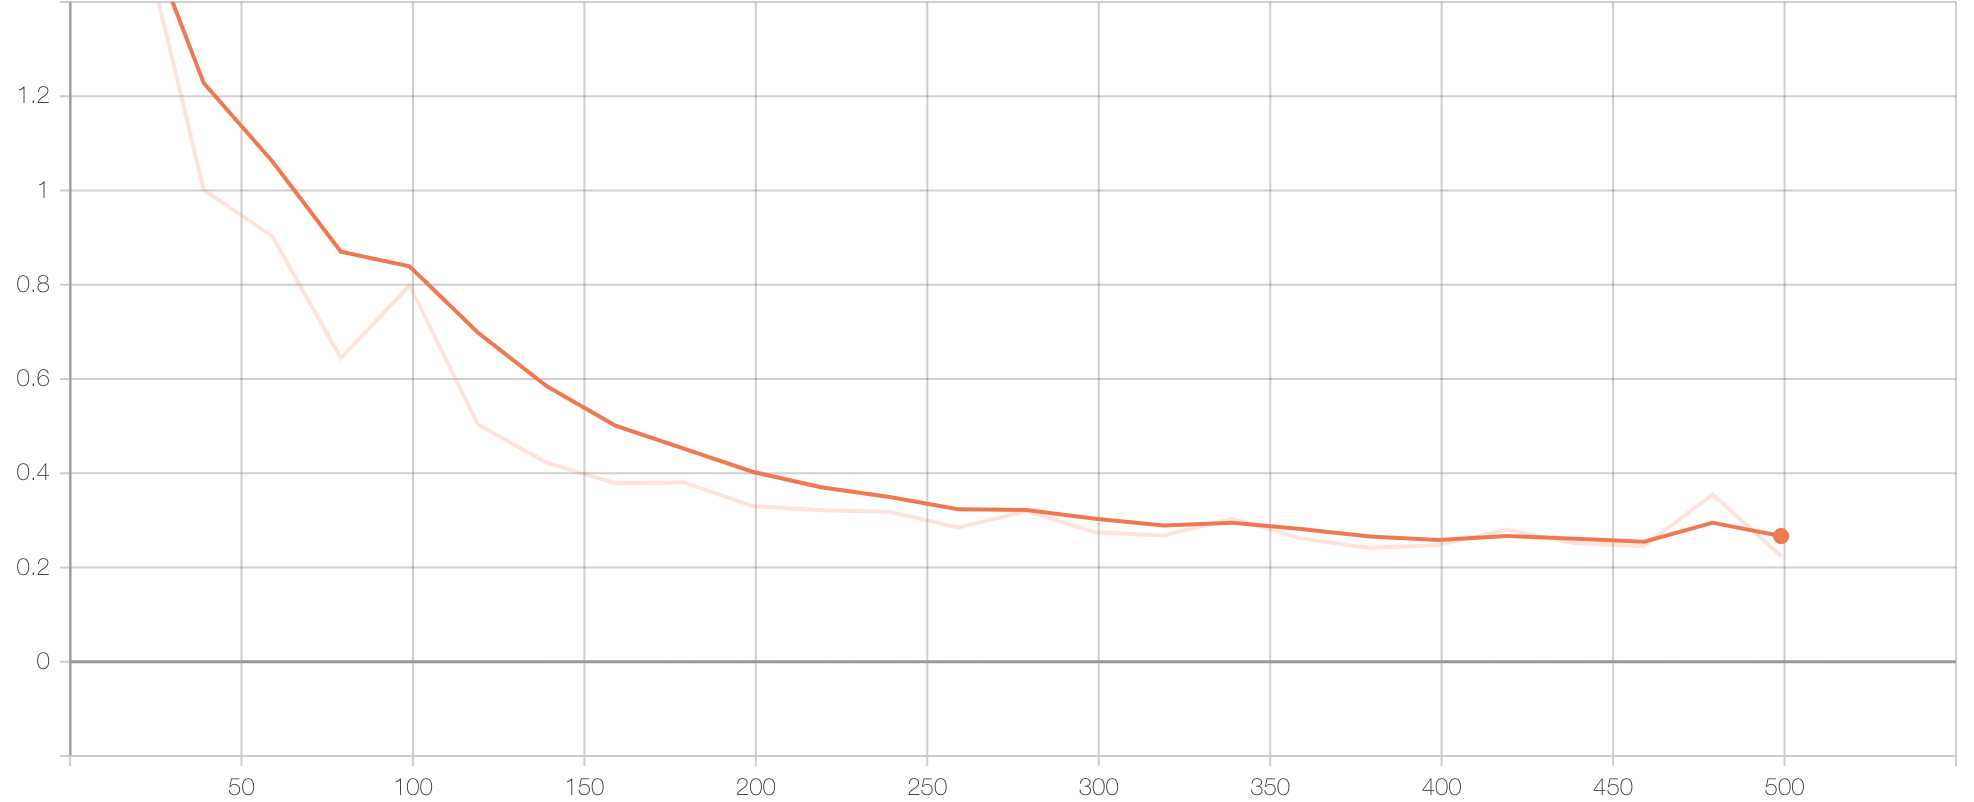
\includegraphics[scale=0.35]{figures/loss_cls_retinanet_4}
\caption{\small \sl «Loss cls», også kjent som «entropy loss», for RetinaNet-modellen. \label{fig:loss_cls_retinanet}}
\end{center}
\end{figure}

Neste graf viser utviklingen av learning rate. Learning rate går stadig nedover ettersom modellen trenes, dette gjøres med en learning rate scheduler. Dette gjøres i et forsøk på å få ned total loss.

\begin{figure}[H]
\begin{center} 
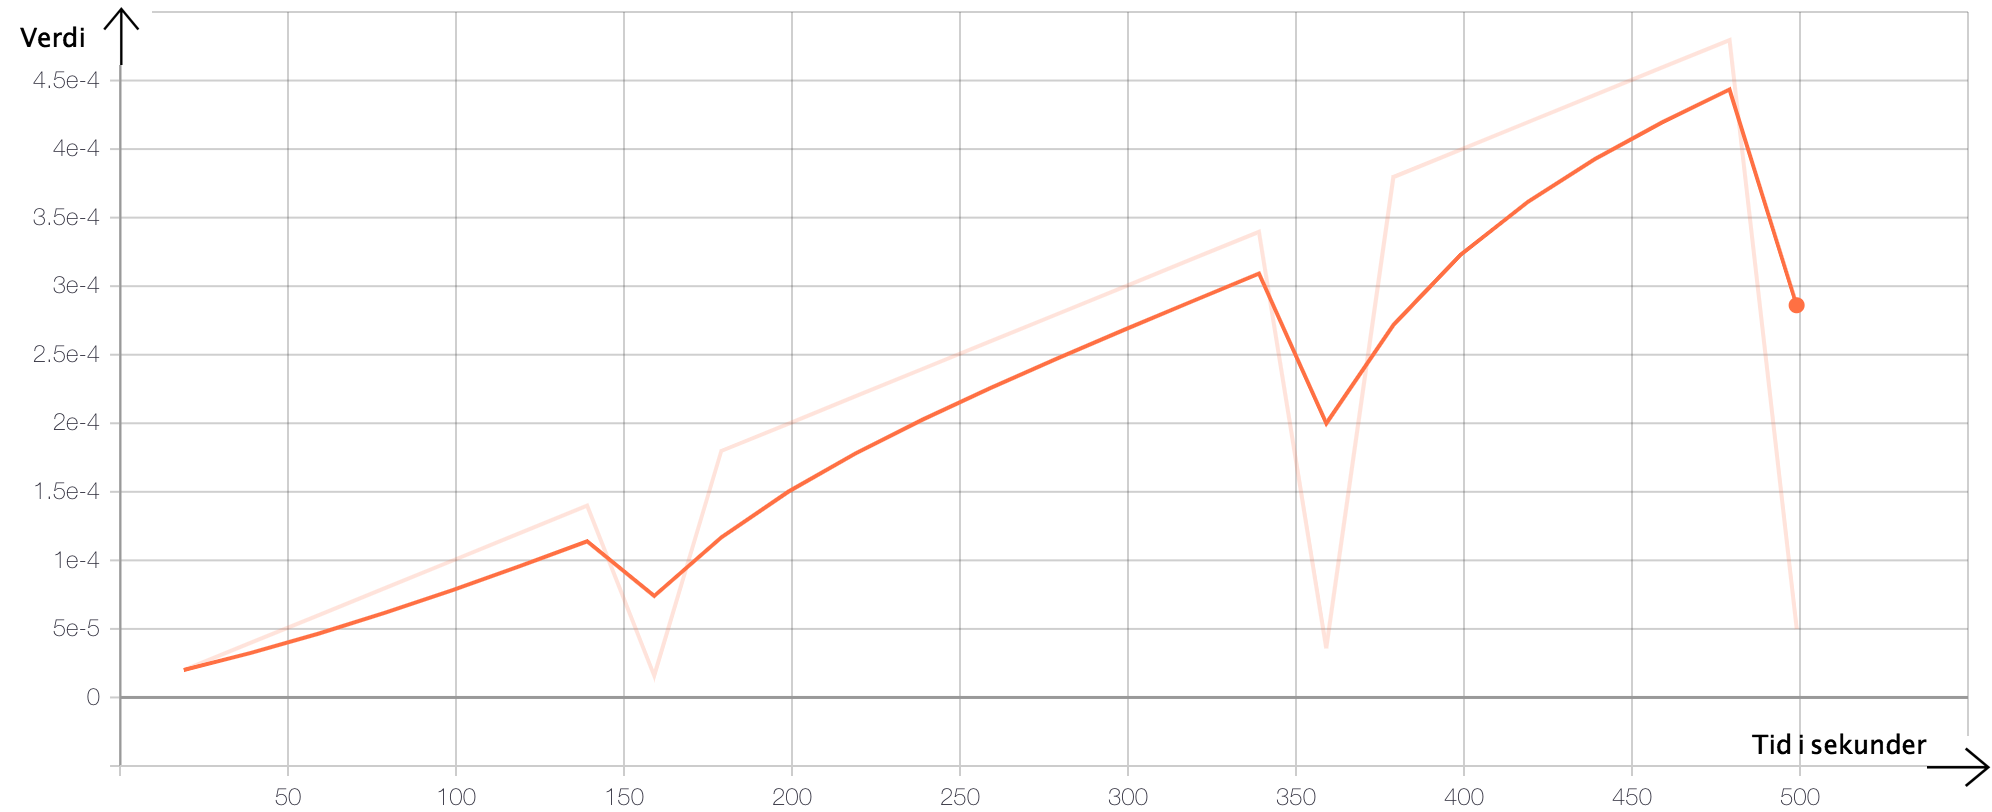
\includegraphics[scale=0.35]{figures/lr_retinanet_5}
\caption{\small \sl Utviklingen av learning rate for RetinaNet-modellen. \label{fig:lr_retinanet}}
\end{center}
\end{figure}

%\begin{figure}[h!]
%\begin{center} 
%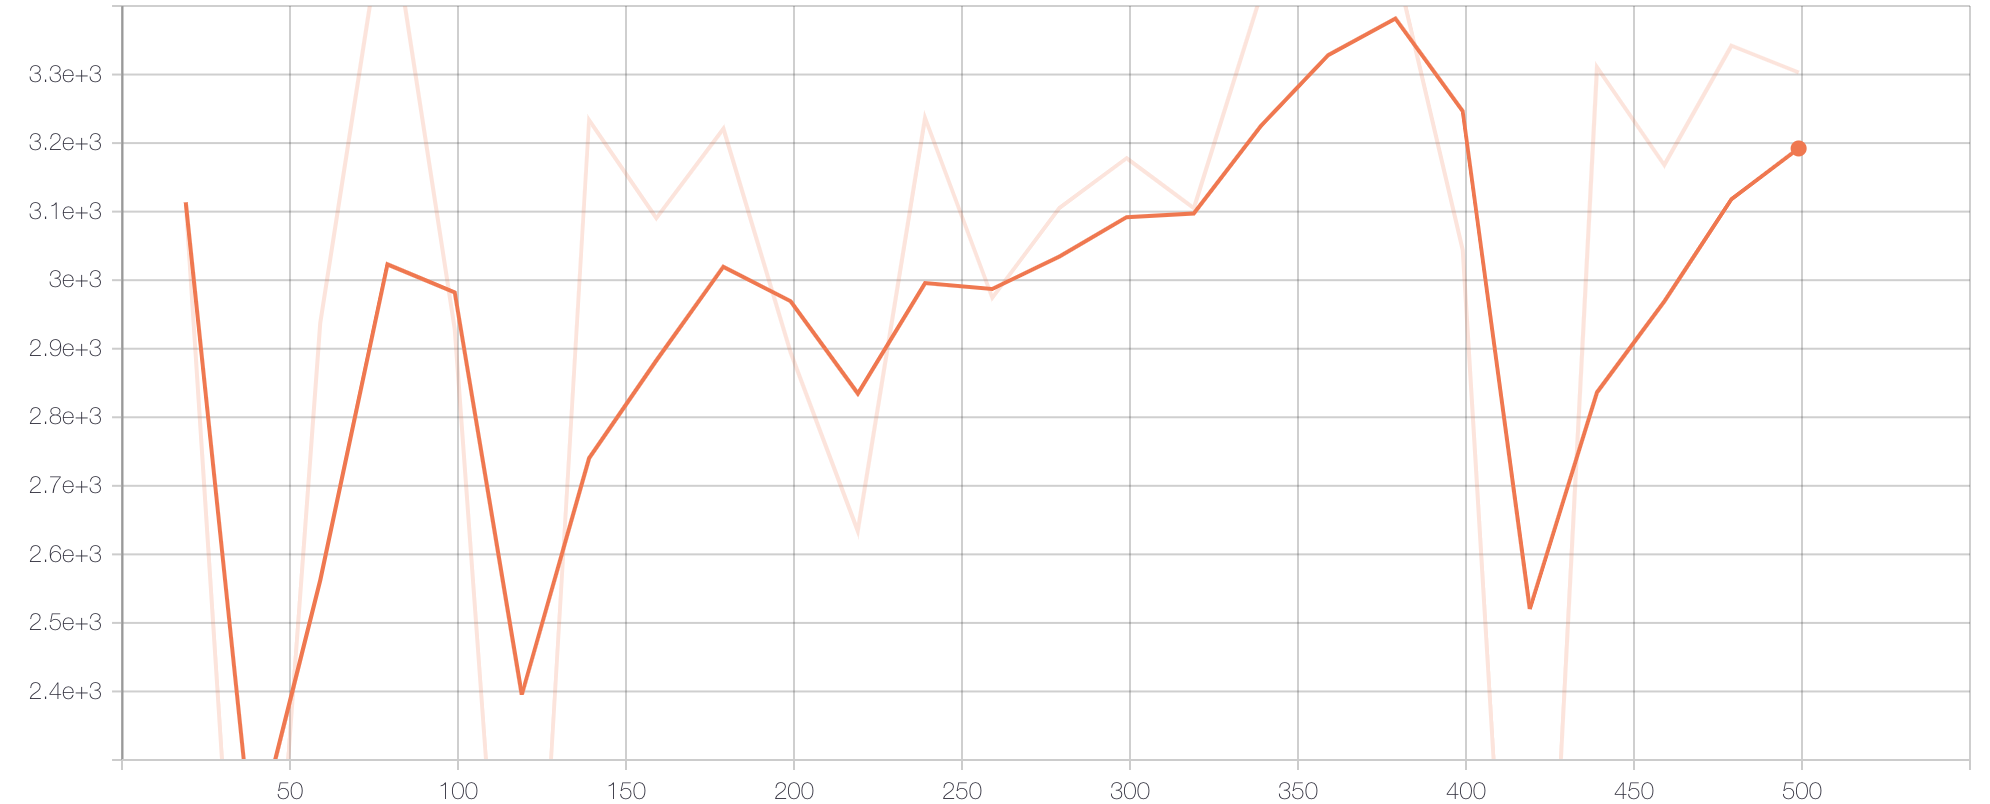
\includegraphics[scale=0.35]{figures/num_foreground_6}
%\caption{\small \sl num foreground RetinaNet. \label{fig:num_foreground}}
%\end{center}
%\end{figure}

%\begin{figure}[h!]
%\begin{center} 
%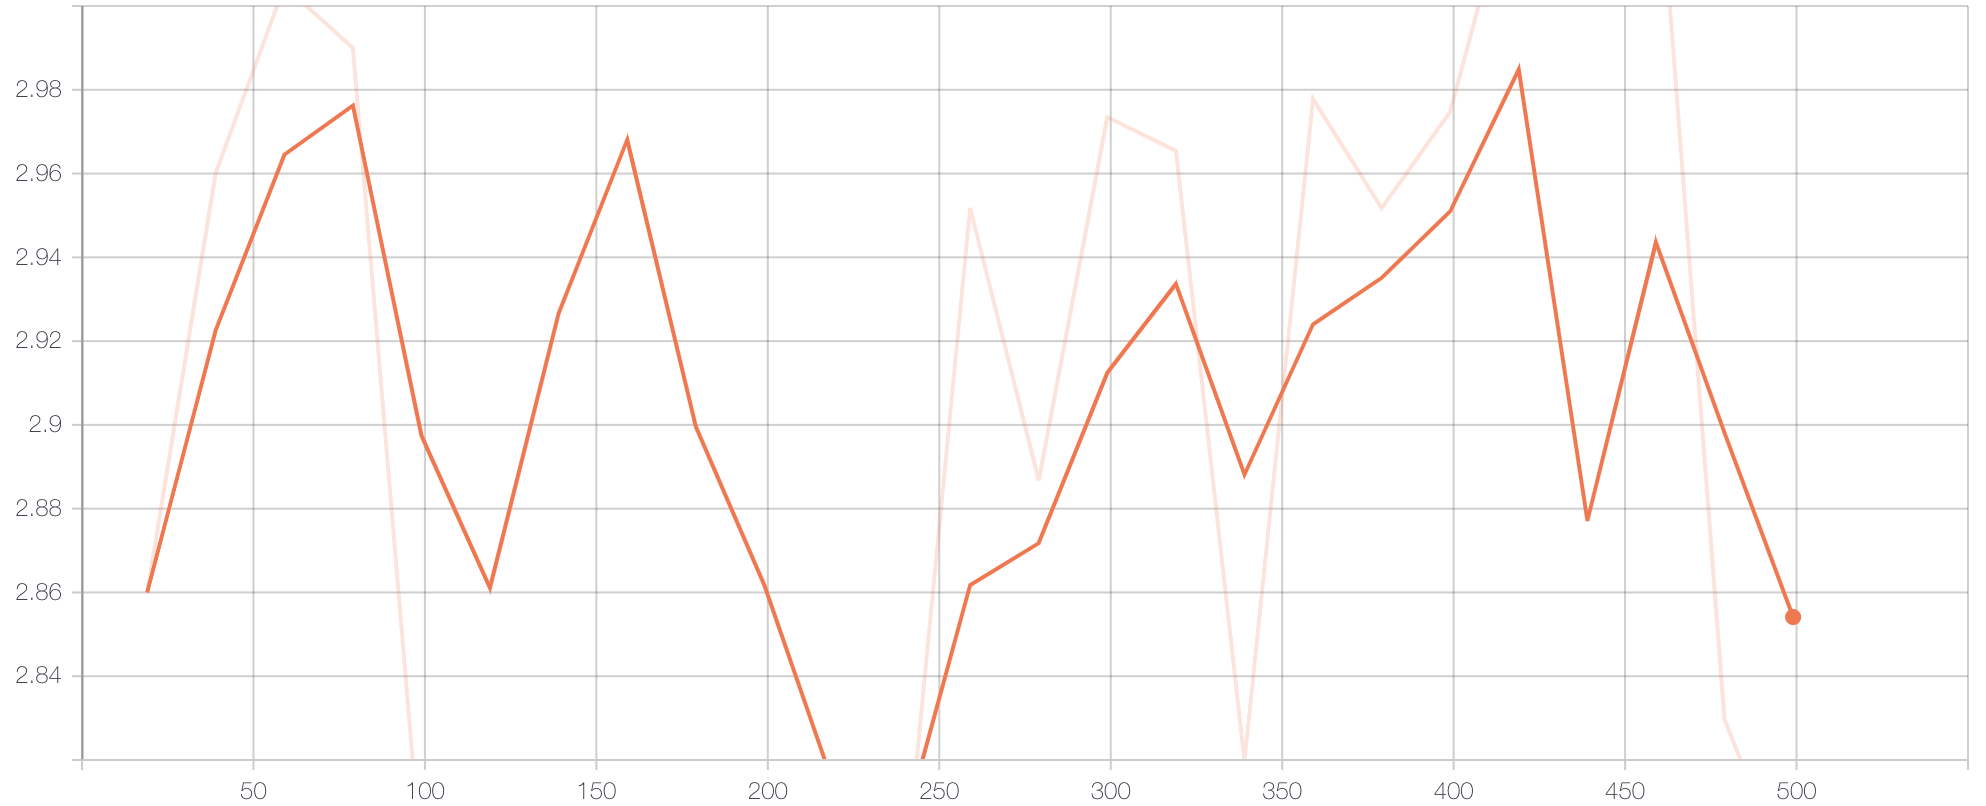
\includegraphics[scale=0.35]{figures/time_retinanet_7}
%\caption{\small \sl time RetinaNet. \label{fig:time_retinanet}}
%\end{center}
%\end{figure}

Den neste grafen viser utviklingen av total loss.

\begin{figure}[H]
\begin{center} 
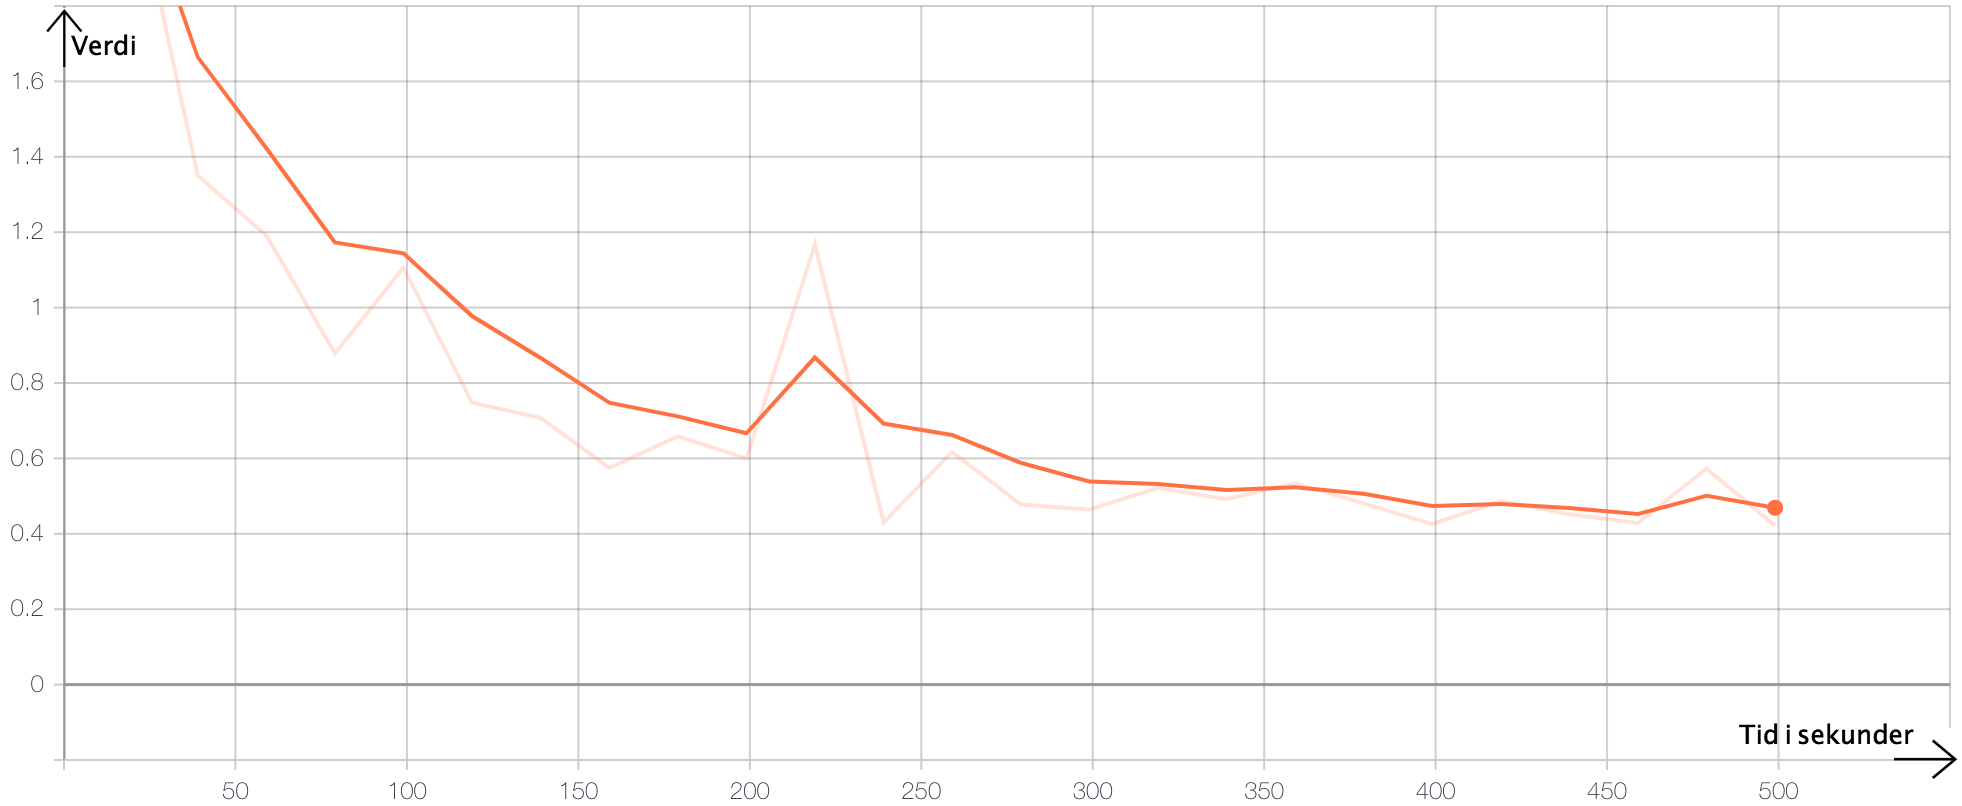
\includegraphics[scale=0.35]{figures/total_loss_retinanet_8}
\caption{\small \sl Total loss for RetinaNet-eksperimentet. \label{fig:total_loss_retinanet}}
\end{center}
\end{figure}

RetinaNet-resultatene for dette eksperimentet er også tilgjengelige på nettet.\footnote{\url{https://tensorboard.dev/experiment/2PxmdvA5QdavQC0YLABdgw}}

\subsection{YOLO}

Når YOLOv4-modellen ble testet på datasettet så hadde modellen en mAP på 73 \%. Se figur \ref{fig:chart_yolo}. Total loss gikk fra 5533,6 ned til litt over 5,5. %When tested on individual source of dataset, the model achieved best results on Wells Dam dataset with 0.5575 mAP, se figur \ref{fig:chart_yolo}. Wells Dam dataset’s better performance than the other two datasets were as expected, considering its high resolution and three full color channels. However, the mAP metric on Wells Dam dataset is lower than our expectation. Fig. 2 F reveals that most of the false detection in Wells Dam dataset are at the side of fish ladder window, where only partial of the fish bodies are visible and difficult for even human annotators to correctly label. These hard cases are sometimes more numerous than fish passing through the white plate, which greatly reduced the overall mAP score on the Wells Dam dataset. \cite{Xu og Matzner 2018}

%mAP (mean average precision) - mean value of average precisions for each class, where average precision is average value of 11 points on PR-curve for each possible threshold (each probability of detection) for the same class (Precision-Recall in terms of PascalVOC, where Precision=TP/(TP+FP) and Recall=TP/(TP+FN) ), %page-11: http://homepages.inf.ed.ac.uk/ckiw/postscript/ijcv_voc09.pdf

\begin{figure}[h!]
\begin{center} 
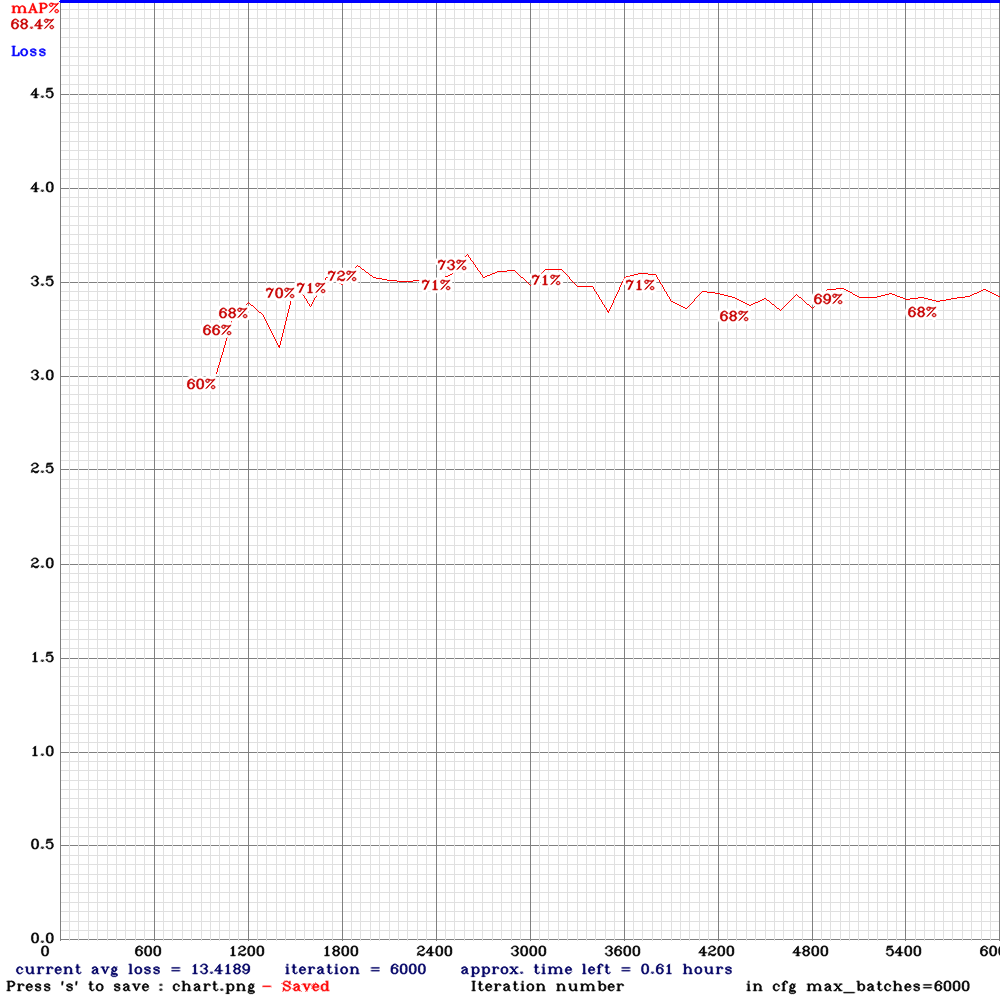
\includegraphics[scale=0.35]{figures/chart_yolo-obj.png}
\caption{\small \sl graf YOLO. \label{fig:chart_yolo}}
\end{center}
\end{figure}